\documentclass[../main.tex]{subfiles}
\graphicspath{{\subfix{../../images/}}}

\begin{document}

Encryption is a process by which data is obfuscated in a certain way that only the sender and receiver can see the data in question, but onlookers along the way cannot. The process of obfuscating is completely reversible given a consensus on which method to use. Two of them exist. In what matters to us, keys are used to achieve this process.

\subsubsection{Symmetric Encryption}

This is when one key is used to encrypt and decrypt the data. The key is applied to the data to encrypt it, and applied to the data to decrypt it. Although the approach is simple, if a hacker gets hold of the key, all data encrypted with the key is compromized.

First, they go to a secure location and exchange their keys. Then, they can exchange data:

\begin{figure}[H]
    \centering
    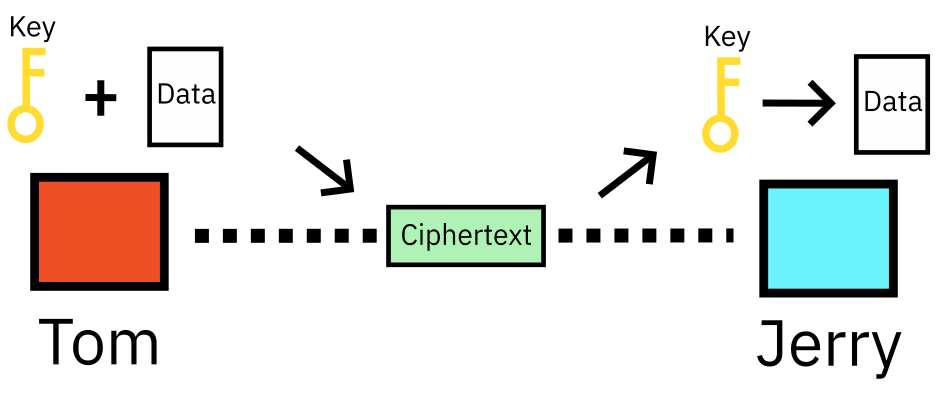
\includegraphics[width=0.7\textwidth]{symmetric.png}
    \caption{Tom and Jerry exchanges a message with the same key.}
    \label{fig:symmetric}
\end{figure}

The same key is used both for encryption and decryption.

\subsubsection{Asymmetric Encryption}

This is when both the sender and the receiver have a pair of keys. One is used to decrypt data (the private key), and the other one is used to encrypt data (the public key). The public key is kept public, as anybody should be able to encrypt data for you. But only yourself can decrypt the data people garbled up for you. This means that only you can decrypt the data, which is the intent. If you want to encrypt data for someone else, you use their public key, and the other person has the private key to decrypt it.

Let's say Tom and Jerry now wants to make use of asymmetric encryption. To begin, they need each other's keys to encrypt data for one another. The process is called a key exchange (self explanatory).

\begin{figure}[H]
    \centering
    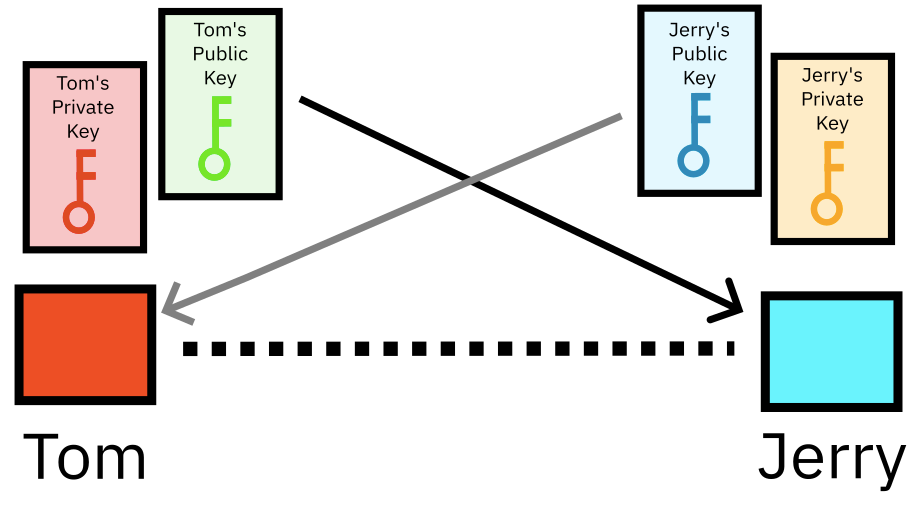
\includegraphics[width=0.7\textwidth]{key_exchange.png}
    \caption{Tom and Jerry exchanges keys.}
    \label{fig:key_exchange}
\end{figure}

Then, if Tom wants to encrypt data for Jerry, Tom uses Jerry's public key, and Jerry decripts it with his private key.

\begin{figure}[H]
    \centering
    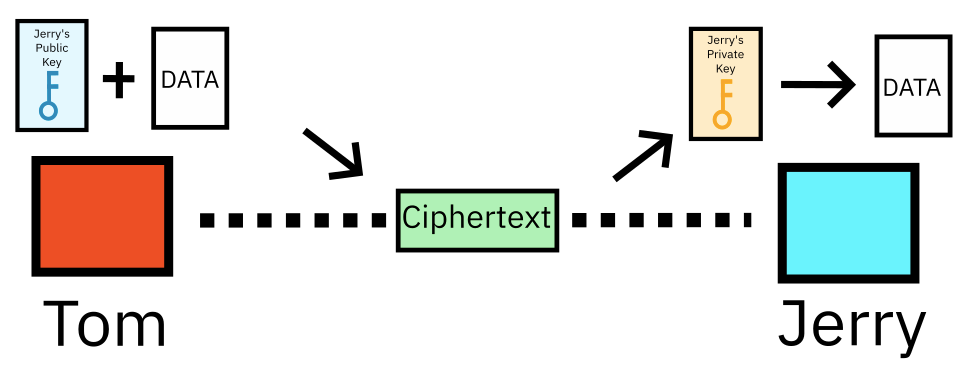
\includegraphics[width=0.7\textwidth]{tom_jerry_exchange.png}
    \caption{Tom sends data to Jerry.}
    \label{fig:tom_jerry_exchange}
\end{figure}

And vice-versa.

\begin{figure}[H]
    \centering
    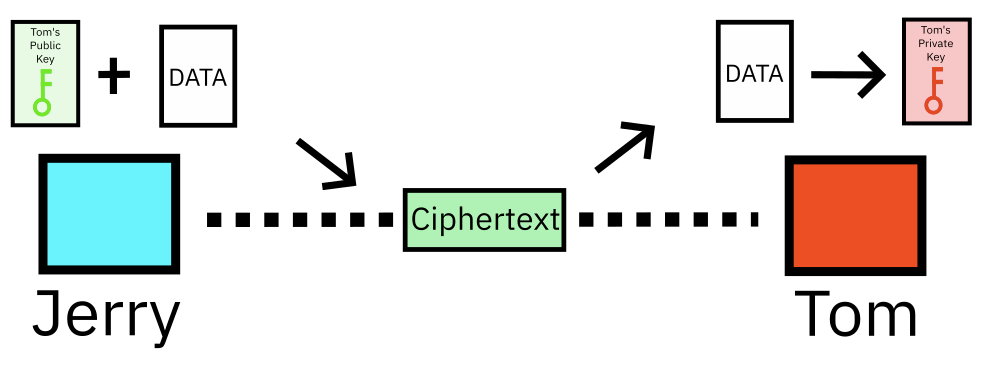
\includegraphics[width=0.7\textwidth]{jerry_tom_exchange.png}
    \caption{Jerry sends data to Tom.}
    \label{fig:jerry_tom_exchange}
\end{figure}

\end{document}
